% Options for packages loaded elsewhere
\PassOptionsToPackage{unicode}{hyperref}
\PassOptionsToPackage{hyphens}{url}
%
\documentclass[
]{article}
\usepackage{amsmath,amssymb}
\usepackage{lmodern}
\usepackage{ifxetex,ifluatex}
\ifnum 0\ifxetex 1\fi\ifluatex 1\fi=0 % if pdftex
  \usepackage[T1]{fontenc}
  \usepackage[utf8]{inputenc}
  \usepackage{textcomp} % provide euro and other symbols
\else % if luatex or xetex
  \usepackage{unicode-math}
  \defaultfontfeatures{Scale=MatchLowercase}
  \defaultfontfeatures[\rmfamily]{Ligatures=TeX,Scale=1}
\fi
% Use upquote if available, for straight quotes in verbatim environments
\IfFileExists{upquote.sty}{\usepackage{upquote}}{}
\IfFileExists{microtype.sty}{% use microtype if available
  \usepackage[]{microtype}
  \UseMicrotypeSet[protrusion]{basicmath} % disable protrusion for tt fonts
}{}
\makeatletter
\@ifundefined{KOMAClassName}{% if non-KOMA class
  \IfFileExists{parskip.sty}{%
    \usepackage{parskip}
  }{% else
    \setlength{\parindent}{0pt}
    \setlength{\parskip}{6pt plus 2pt minus 1pt}}
}{% if KOMA class
  \KOMAoptions{parskip=half}}
\makeatother
\usepackage{xcolor}
\IfFileExists{xurl.sty}{\usepackage{xurl}}{} % add URL line breaks if available
\IfFileExists{bookmark.sty}{\usepackage{bookmark}}{\usepackage{hyperref}}
\hypersetup{
  pdftitle={LIN 380 Coursebook},
  pdfauthor={Jerid Francom},
  hidelinks,
  pdfcreator={LaTeX via pandoc}}
\urlstyle{same} % disable monospaced font for URLs
\usepackage[margin=1in]{geometry}
\usepackage{color}
\usepackage{fancyvrb}
\newcommand{\VerbBar}{|}
\newcommand{\VERB}{\Verb[commandchars=\\\{\}]}
\DefineVerbatimEnvironment{Highlighting}{Verbatim}{commandchars=\\\{\}}
% Add ',fontsize=\small' for more characters per line
\usepackage{framed}
\definecolor{shadecolor}{RGB}{248,248,248}
\newenvironment{Shaded}{\begin{snugshade}}{\end{snugshade}}
\newcommand{\AlertTok}[1]{\textcolor[rgb]{0.94,0.16,0.16}{#1}}
\newcommand{\AnnotationTok}[1]{\textcolor[rgb]{0.56,0.35,0.01}{\textbf{\textit{#1}}}}
\newcommand{\AttributeTok}[1]{\textcolor[rgb]{0.77,0.63,0.00}{#1}}
\newcommand{\BaseNTok}[1]{\textcolor[rgb]{0.00,0.00,0.81}{#1}}
\newcommand{\BuiltInTok}[1]{#1}
\newcommand{\CharTok}[1]{\textcolor[rgb]{0.31,0.60,0.02}{#1}}
\newcommand{\CommentTok}[1]{\textcolor[rgb]{0.56,0.35,0.01}{\textit{#1}}}
\newcommand{\CommentVarTok}[1]{\textcolor[rgb]{0.56,0.35,0.01}{\textbf{\textit{#1}}}}
\newcommand{\ConstantTok}[1]{\textcolor[rgb]{0.00,0.00,0.00}{#1}}
\newcommand{\ControlFlowTok}[1]{\textcolor[rgb]{0.13,0.29,0.53}{\textbf{#1}}}
\newcommand{\DataTypeTok}[1]{\textcolor[rgb]{0.13,0.29,0.53}{#1}}
\newcommand{\DecValTok}[1]{\textcolor[rgb]{0.00,0.00,0.81}{#1}}
\newcommand{\DocumentationTok}[1]{\textcolor[rgb]{0.56,0.35,0.01}{\textbf{\textit{#1}}}}
\newcommand{\ErrorTok}[1]{\textcolor[rgb]{0.64,0.00,0.00}{\textbf{#1}}}
\newcommand{\ExtensionTok}[1]{#1}
\newcommand{\FloatTok}[1]{\textcolor[rgb]{0.00,0.00,0.81}{#1}}
\newcommand{\FunctionTok}[1]{\textcolor[rgb]{0.00,0.00,0.00}{#1}}
\newcommand{\ImportTok}[1]{#1}
\newcommand{\InformationTok}[1]{\textcolor[rgb]{0.56,0.35,0.01}{\textbf{\textit{#1}}}}
\newcommand{\KeywordTok}[1]{\textcolor[rgb]{0.13,0.29,0.53}{\textbf{#1}}}
\newcommand{\NormalTok}[1]{#1}
\newcommand{\OperatorTok}[1]{\textcolor[rgb]{0.81,0.36,0.00}{\textbf{#1}}}
\newcommand{\OtherTok}[1]{\textcolor[rgb]{0.56,0.35,0.01}{#1}}
\newcommand{\PreprocessorTok}[1]{\textcolor[rgb]{0.56,0.35,0.01}{\textit{#1}}}
\newcommand{\RegionMarkerTok}[1]{#1}
\newcommand{\SpecialCharTok}[1]{\textcolor[rgb]{0.00,0.00,0.00}{#1}}
\newcommand{\SpecialStringTok}[1]{\textcolor[rgb]{0.31,0.60,0.02}{#1}}
\newcommand{\StringTok}[1]{\textcolor[rgb]{0.31,0.60,0.02}{#1}}
\newcommand{\VariableTok}[1]{\textcolor[rgb]{0.00,0.00,0.00}{#1}}
\newcommand{\VerbatimStringTok}[1]{\textcolor[rgb]{0.31,0.60,0.02}{#1}}
\newcommand{\WarningTok}[1]{\textcolor[rgb]{0.56,0.35,0.01}{\textbf{\textit{#1}}}}
\usepackage{longtable,booktabs,array}
\usepackage{calc} % for calculating minipage widths
% Correct order of tables after \paragraph or \subparagraph
\usepackage{etoolbox}
\makeatletter
\patchcmd\longtable{\par}{\if@noskipsec\mbox{}\fi\par}{}{}
\makeatother
% Allow footnotes in longtable head/foot
\IfFileExists{footnotehyper.sty}{\usepackage{footnotehyper}}{\usepackage{footnote}}
\makesavenoteenv{longtable}
\usepackage{graphicx}
\makeatletter
\def\maxwidth{\ifdim\Gin@nat@width>\linewidth\linewidth\else\Gin@nat@width\fi}
\def\maxheight{\ifdim\Gin@nat@height>\textheight\textheight\else\Gin@nat@height\fi}
\makeatother
% Scale images if necessary, so that they will not overflow the page
% margins by default, and it is still possible to overwrite the defaults
% using explicit options in \includegraphics[width, height, ...]{}
\setkeys{Gin}{width=\maxwidth,height=\maxheight,keepaspectratio}
% Set default figure placement to htbp
\makeatletter
\def\fps@figure{htbp}
\makeatother
% Make links footnotes instead of hotlinks:
\DeclareRobustCommand{\href}[2]{#2\footnote{\url{#1}}}
\setlength{\emergencystretch}{3em} % prevent overfull lines
\providecommand{\tightlist}{%
  \setlength{\itemsep}{0pt}\setlength{\parskip}{0pt}}
\setcounter{secnumdepth}{5}
% default
\usepackage{booktabs}
\usepackage{amsthm}
\usepackage{float}
\makeatletter
\def\thm@space@setup{%
  \thm@preskip=8pt plus 2pt minus 4pt
  \thm@postskip=\thm@preskip
}
\makeatother

% added
\usepackage{longtable}
\usepackage{framed,color}
\definecolor{shadecolor}{RGB}{248,248,248}

\ifxetex
  \usepackage{letltxmacro}
  \setlength{\XeTeXLinkMargin}{2pt}
  \LetLtxMacro\SavedIncludeGraphics\includegraphics
  \def\includegraphics#1#{% #1 catches optional stuff (star/opt. arg.)
    \IncludeGraphicsAux{#1}%
  }%
  \newcommand*{\IncludeGraphicsAux}[2]{%
    \XeTeXLinkBox{%
      \SavedIncludeGraphics#1{#2}%
    }%
  }%
\fi

\newenvironment{rmdblock}[1]
  {\begin{shaded*}
  \begin{itemize}
  \renewcommand{\labelitemi}{
    \raisebox{-.5\height}[0pt][0pt]{
      {\setkeys{Gin}{width=2em,keepaspectratio}\includegraphics{assets/images/#1}}
    }
  }
  \item
  }
  {
  \end{itemize}
  \end{shaded*}
  }
\newenvironment{rmdkey}
  {\begin{rmdblock}{key}}
  {\end{rmdblock}}
\newenvironment{rmdnote}
  {\begin{rmdblock}{note}}
  {\end{rmdblock}}
\newenvironment{rmdtip}
  {\begin{rmdblock}{tip}}
  {\end{rmdblock}}
\newenvironment{rmdwarning}
  {\begin{rmdblock}{warning}}
  {\end{rmdblock}}
\newenvironment{rmdactivity}
  {\begin{rmdblock}{code}}
  {\end{rmdblock}}

\ifluatex
  \usepackage{selnolig}  % disable illegal ligatures
\fi
\usepackage[]{natbib}
\bibliographystyle{apalike}

\title{LIN 380 Coursebook}
\usepackage{etoolbox}
\makeatletter
\providecommand{\subtitle}[1]{% add subtitle to \maketitle
  \apptocmd{\@title}{\par {\large #1 \par}}{}{}
}
\makeatother
\subtitle{Text as Data: An introduction to quantative text analysis and reproducible research with R}
\author{Jerid Francom}
\date{April 22, 2021 (latest version)}

\begin{document}
\maketitle

{
\setcounter{tocdepth}{2}
\tableofcontents
}
\hypertarget{about}{%
\section*{About}\label{about}}
\addcontentsline{toc}{section}{About}

\ldots{}

\hypertarget{todos}{%
\subsection*{TODOs}\label{todos}}
\addcontentsline{toc}{subsection}{TODOs}

\begin{itemize}
\tightlist
\item
  Consider creating an R cheat sheet for text analytics in R. \href{https://www.rstudio.com/resources/cheatsheets/how-to-contribute-a-cheatsheet/}{templates for creating cheat sheets}, \href{https://www.rstudio.com/resources/cheatsheets/}{examples}
\item
  \ldots{}
\end{itemize}

\hypertarget{build-and-session-information}{%
\subsection*{Build and session information}\label{build-and-session-information}}
\addcontentsline{toc}{subsection}{Build and session information}

This coursebook was written in \href{http://bookdown.org/}{bookdown} inside \href{http://www.rstudio.com/ide/}{RStudio}. The website is hosted with \href{https://pages.github.com/}{GitHub Pages} and the complete source is available from \href{https://github.com/francojc}{GitHub}.

This version of the coursebook was built with:

\begin{verbatim}
#> Finding R package dependencies ... Done!
#>  setting  value                       
#>  version  R version 4.0.2 (2020-06-22)
#>  os       macOS  10.16                
#>  system   x86_64, darwin17.0          
#>  ui       X11                         
#>  language (EN)                        
#>  collate  en_US.UTF-8                 
#>  ctype    en_US.UTF-8                 
#>  tz       America/New_York            
#>  date     2021-04-22
\end{verbatim}

And depends on these packages:

\textbackslash begin\{center\}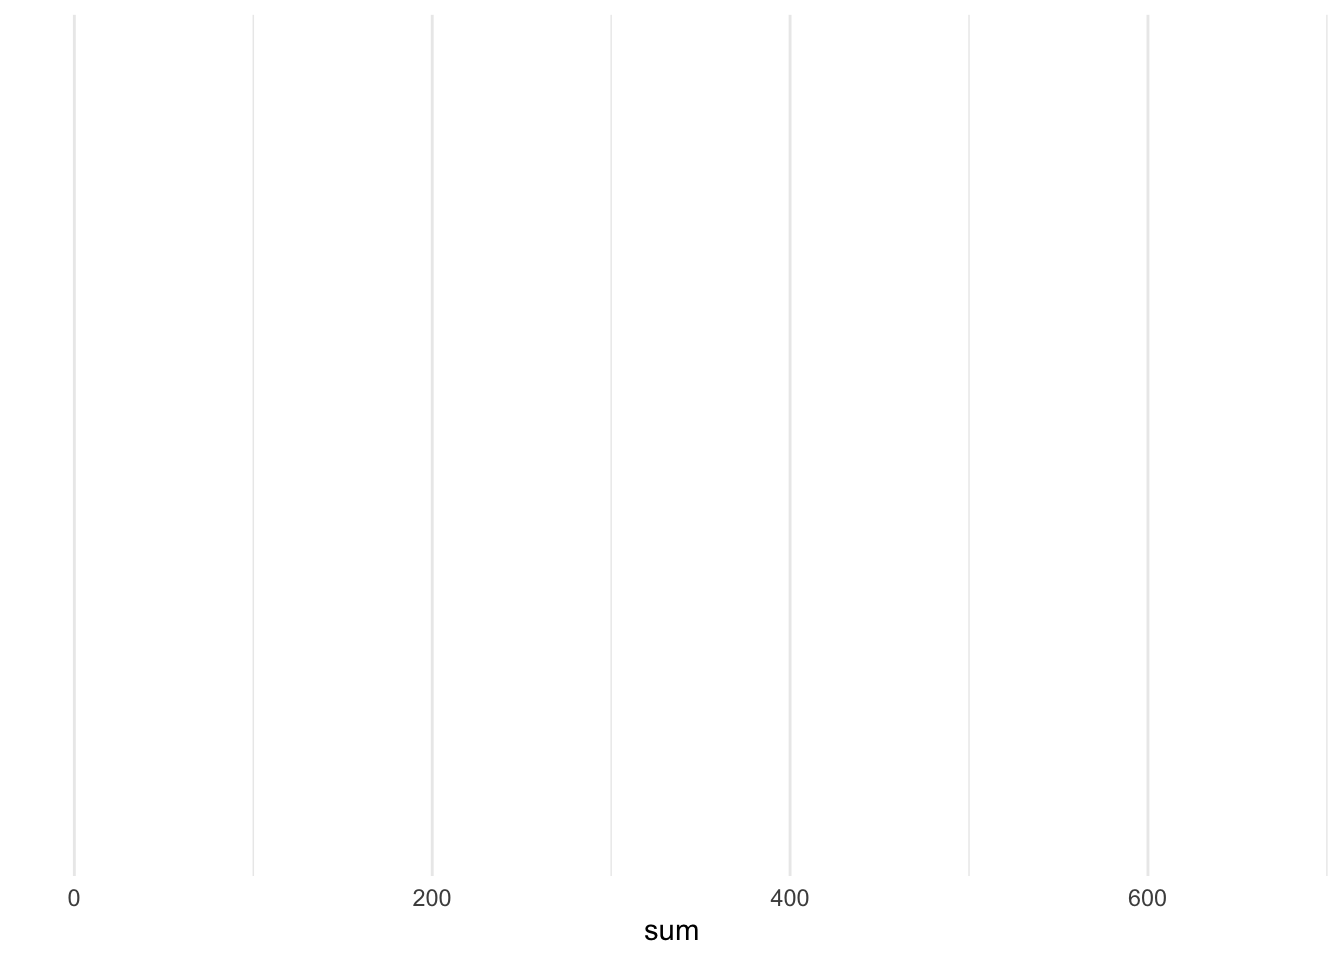
\includegraphics[width=0.7\linewidth]{index_files/figure-latex/unnamed-chunk-3-1}

\hypertarget{part-welcome}{%
\part{Welcome}\label{part-welcome}}

\hypertarget{course-overview}{%
\section*{Overview}\label{course-overview}}
\addcontentsline{toc}{section}{Overview}

\textbf{WELCOME}

\ldots{} overview text

\textbf{Learning outcomes}

\begin{itemize}
\tightlist
\item
  PS (2) demonstrate ability to produce collaborative and reproducible research using R, RStudio, and GitHub
\end{itemize}

\textbf{Learning goals}

\begin{itemize}
\tightlist
\item
  \ldots{}
\end{itemize}

\hypertarget{about-this-coursebook}{%
\section*{About this coursebook}\label{about-this-coursebook}}
\addcontentsline{toc}{section}{About this coursebook}

In recent years there has been a growing buzz around the term `Data Science' and related terms; data analytics, data mining, \emph{etc}. In a nutshell data science is the process by which an investigator leverages statistical methods and computational power to uncover insight from large datasets. Driven in large part by the increase in computing power available to the average individual and the increasing amount of electronic data that is now available through the internet, interest in data science has expanded to virtually all fields in academia and areas in the public sector. Data scientists are in high demand and this trend is expected to continue into the foreseeable future, which means that undergraduate and post-graduate students will be increasingly seeking out resources and training in the area.

This coursebook is an introduction to the fundamental concepts and practical programming skills from Data Science that are increasingly employed in a variety of language-centered fields and sub-fields. It is geared towards advanced undergraduates and graduate students of linguistics and related fields. As quantitative research skills are quickly becoming a core aspect of many language programs, this coursebook aims to provide a fundamental understanding of theoretical concepts, programming skills, and statistical methods for doing quantitative text analysis. Through these skills we will explore topics and replicate previous research in a variety of areas in language research (psycholinguistics, sociolinguistics, translation studies, \emph{etc.}) using common methods and authentic data sources.

No programming knowledge is assumed, either with R or otherwise.

\hypertarget{approach}{%
\subsection*{Approach}\label{approach}}
\addcontentsline{toc}{subsection}{Approach}

Many textbooks on doing `Data Science', even those that have a domain-centric approach, such as text analysis, tend to focus on the basic `tidy' approach, seen in Figure \ref{fig:tidy-workflow-img}. to analysis and do not tend to encourage readers to lead with research questions. A big part, or perhaps the biggest part of doing quantitative research, and research in general is what is the question to be addressed. Then comes how to orient the research approach to best address this question (or questions). Then we move on to matching data sources, organizing data, modeling data, and finally reporting findings

\begin{figure}

{\centering 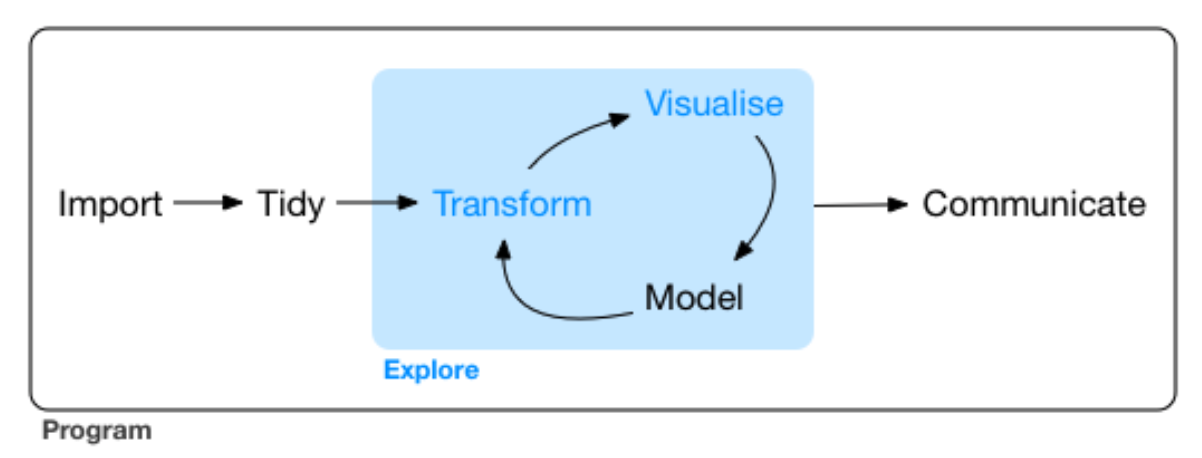
\includegraphics[width=0.7\linewidth]{images/preface-tidy-approach} 

}

\caption{Wickham diagram...}\label{fig:tidy-workflow-img}
\end{figure}

I think a central advantage to this coursebook for language researchers is to thread the project goals without technical implementation in mind first.

Then, after a general idea about what the data should look like, how it should be analyzed, and how the analysis will contribute to knowledge in the field, we can move towards implementing these preliminary formulations in R code. In a way this is the classic separation between content and format --the content of our research should precede the format it should or will take.

\hypertarget{conventions}{%
\subsection*{Conventions}\label{conventions}}
\addcontentsline{toc}{subsection}{Conventions}

This coursebook is about the concepts for understanding and the techniques for doing quantitative text analysis with R. Therefore there will be an intermingling of prose and code presented. As such, an attempt to establish consistent conventions throughout the text has been made to signal reader's attention as appropriate. As we explore concepts, R code itself will be incorporated into the text. This may be a unique textbook compared to others you have seen. It has been created using R itself --specifically using an R language package called \texttt{bookdown} \citep{R-bookdown}. This R package makes it possible to write, execute (`run'), and display code and results within the text.

For example, the following text block shows actual R code and the results that are generated when running this code. Note that the hashtag \texttt{\#} signals a \textbf{code comment}. The code follows within the same text block and a subsequent text block displays the output of the code.

\begin{Shaded}
\begin{Highlighting}[]
\CommentTok{\# Add 1 plus 1}
\DecValTok{1} \SpecialCharTok{+} \DecValTok{1}
\CommentTok{\#\textgreater{} [1] 2}
\end{Highlighting}
\end{Shaded}

Inline code will be used when code blocks are short and the results are not needed for display. For example, the same code as above will sometimes appear as \texttt{1\ +\ 1}.

When necessary meta-description of code will appear. This is particularly relevant for R Markdown documents.

\begin{verbatim}
```{r test-code}
1 + 1
```
\end{verbatim}

In terms of prose, key concepts will be signaled using \textbf{\emph{bold italics}}. Terms that appear in this typeface will also appear in the {[}glossary{]} at the end of the text. Furthermore, there are four pose text blocks that will be used to signal the reader's attention: \emph{key points}, \emph{notes}, \emph{tips}, and \emph{warnings}.

Key points summarize the main points to be covered in a chapter or a subsection of the text.

\begin{rmdkey}
In this chapter you will learn:

\begin{itemize}
\tightlist
\item
  the goals of this textbook
\item
  the reasoning for using the R programming language
\item
  important text conventions employed in this textbook
\end{itemize}
\end{rmdkey}

Notes provide a bit more information on the topic or where to find more information.

\begin{rmdnote}
R is more than a powerful statistical programming language, it also can
be used to perform all the necessary steps in a data science project;
including reporting. A relatively new addition to the reporting
capabilities of R is the \texttt{bookdown} package (this textbook was
created using this very package). You can find out more
\href{https://bookdown.org/}{here}.
\end{rmdnote}

Tips are used to signal helpful hints that might otherwise be overlooked.

\begin{rmdtip}
During a the course of an exploratory work session, many R objects are
often created to test ideas. At some point inspecting the workspace
becomes difficult due to the number of objects displayed using
\texttt{ls()}.

To remove all objects from the workspace, use
\texttt{rm(list\ =\ ls())}.
\end{rmdtip}

Errors will be an inevitable part of learning, but some errors can be avoided. The text will used the warning text block to highlight typical pitfalls and errors.

\begin{rmdwarning}
Hello world!\\
This is a warning.
\end{rmdwarning}

Although this is not intended to be a in-depth introduction to statistical techniques, mathematical formulas will be included in the text. These formulas will appear either inline \(1 + 1 = 2\) or as block equations.

\begin{equation}
  \hat{c} = \underset{c \in C} {\mathrm{argmax}} ~\hat{P}(c) \prod_i \hat{P}(w_i|c)
  \label{eq:example-formula}
\end{equation}

Data analysis leans heavily on graphical representations. Figures will appear numbered, as in Figure \ref{fig:test-fig}.

\begin{Shaded}
\begin{Highlighting}[]
\FunctionTok{library}\NormalTok{(ggplot2) }\CommentTok{\# load graphics package}
\FunctionTok{ggplot}\NormalTok{(mtcars, }\FunctionTok{aes}\NormalTok{(}\AttributeTok{x =}\NormalTok{ hp, }\AttributeTok{y =}\NormalTok{ mpg)) }\SpecialCharTok{+} \CommentTok{\# map \textquotesingle{}hp\textquotesingle{} and \textquotesingle{}mpg\textquotesingle{} to coordinate space}
  \FunctionTok{geom\_point}\NormalTok{() }\SpecialCharTok{+} \CommentTok{\# add points}
  \FunctionTok{geom\_smooth}\NormalTok{(}\AttributeTok{method =} \StringTok{"lm"}\NormalTok{) }\SpecialCharTok{+} \CommentTok{\# draw linear trend line}
  \FunctionTok{labs}\NormalTok{(}\AttributeTok{x =} \StringTok{"Horsepower"}\NormalTok{, }\CommentTok{\# label x axis}
       \AttributeTok{y =} \StringTok{"Miles per gallon"}\NormalTok{, }\CommentTok{\# label y axis}
       \AttributeTok{title =} \StringTok{"Test plot"}\NormalTok{, }\CommentTok{\# add title}
       \AttributeTok{subtitle =} \StringTok{"From mtcars dataset"}\NormalTok{) }\CommentTok{\# add subtitle}
\end{Highlighting}
\end{Shaded}

\begin{figure}

{\centering 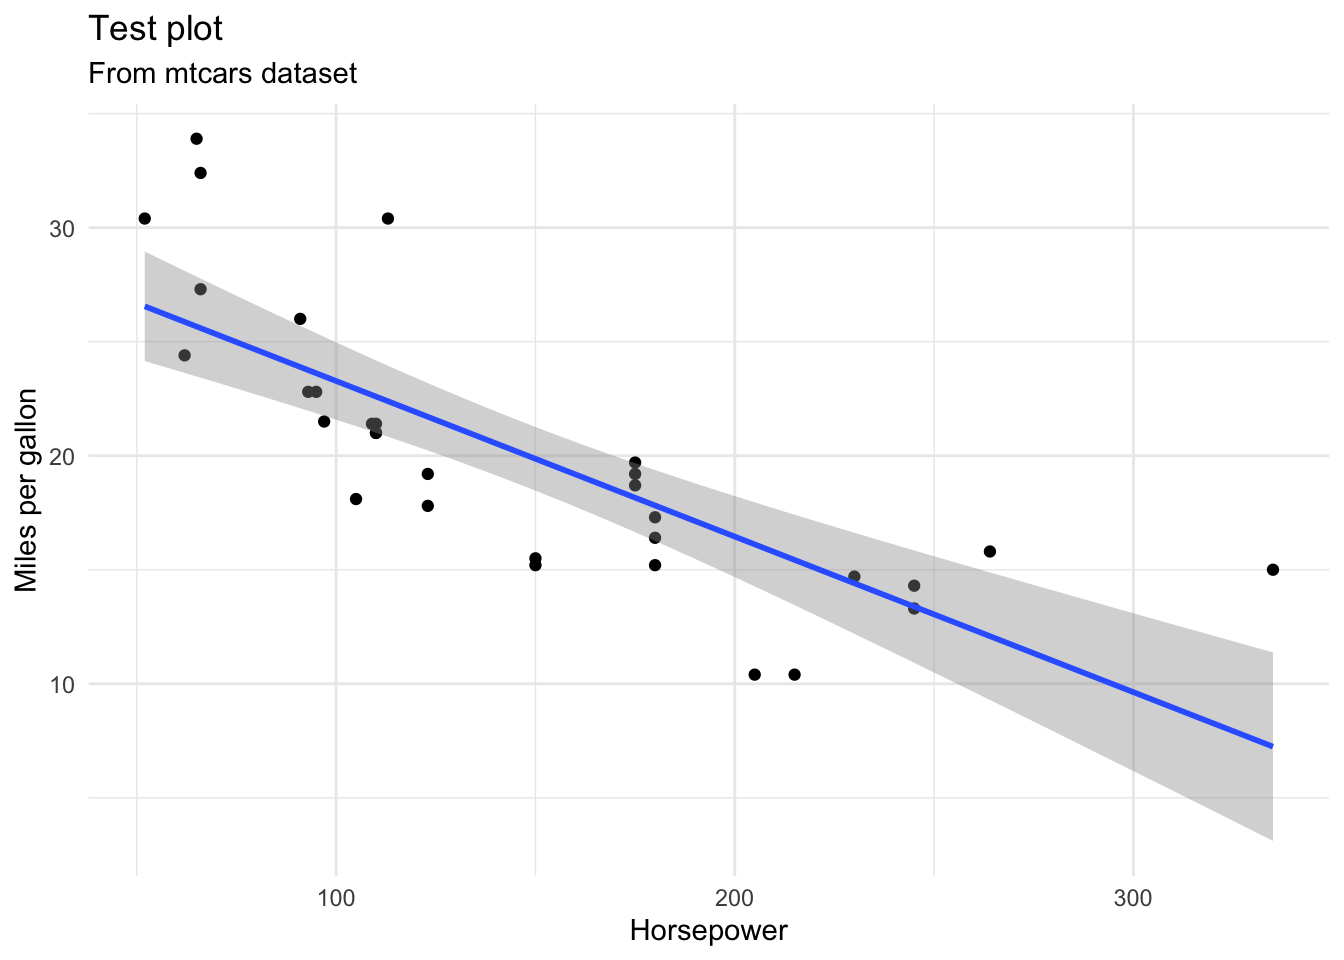
\includegraphics[width=0.7\linewidth]{01-course_files/figure-latex/test-fig-1} 

}

\caption{Test plot from mtcars dataset}\label{fig:test-fig}
\end{figure}

Tables, such as Table \ref{tab:test-tab} will be numbered separately from figures.

\begin{Shaded}
\begin{Highlighting}[]
\NormalTok{knitr}\SpecialCharTok{::}\FunctionTok{kable}\NormalTok{(}\FunctionTok{head}\NormalTok{(iris, }\DecValTok{20}\NormalTok{), }\AttributeTok{caption =} \StringTok{"Here is a nice table!"}\NormalTok{, }\AttributeTok{booktabs =} \ConstantTok{TRUE}\NormalTok{)}
\end{Highlighting}
\end{Shaded}

\begin{table}

\caption{\label{tab:test-tab}Here is a nice table!}
\centering
\begin{tabular}[t]{rrrrl}
\toprule{}
Sepal.Length & Sepal.Width & Petal.Length & Petal.Width & Species\\
\midrule{}
5.1 & 3.5 & 1.4 & 0.2 & setosa\\
4.9 & 3.0 & 1.4 & 0.2 & setosa\\
4.7 & 3.2 & 1.3 & 0.2 & setosa\\
4.6 & 3.1 & 1.5 & 0.2 & setosa\\
5.0 & 3.6 & 1.4 & 0.2 & setosa\\
\addlinespace
5.4 & 3.9 & 1.7 & 0.4 & setosa\\
4.6 & 3.4 & 1.4 & 0.3 & setosa\\
5.0 & 3.4 & 1.5 & 0.2 & setosa\\
4.4 & 2.9 & 1.4 & 0.2 & setosa\\
4.9 & 3.1 & 1.5 & 0.1 & setosa\\
\addlinespace
5.4 & 3.7 & 1.5 & 0.2 & setosa\\
4.8 & 3.4 & 1.6 & 0.2 & setosa\\
4.8 & 3.0 & 1.4 & 0.1 & setosa\\
4.3 & 3.0 & 1.1 & 0.1 & setosa\\
5.8 & 4.0 & 1.2 & 0.2 & setosa\\
\addlinespace
5.7 & 4.4 & 1.5 & 0.4 & setosa\\
5.4 & 3.9 & 1.3 & 0.4 & setosa\\
5.1 & 3.5 & 1.4 & 0.3 & setosa\\
5.7 & 3.8 & 1.7 & 0.3 & setosa\\
5.1 & 3.8 & 1.5 & 0.3 & setosa\\
\bottomrule{}
\end{tabular}
\end{table}

\hypertarget{r-and-rstudio}{%
\section*{R and RStudio}\label{r-and-rstudio}}
\addcontentsline{toc}{section}{R and RStudio}

\hypertarget{git-and-github}{%
\section*{Git and GitHub}\label{git-and-github}}
\addcontentsline{toc}{section}{Git and GitHub}

\citep{Bryan2017a}

\hypertarget{part-foundations}{%
\part{Foundations}\label{part-foundations}}

\hypertarget{foundations-overview}{%
\section*{Overview}\label{foundations-overview}}
\addcontentsline{toc}{section}{Overview}

\textbf{FOUNDATIONS}

In this section the aim is to (1) provide an overview of quantitative research and their applications, by both highlighting visible applications and notable research in various fields. (2) We will under the hood a bit and consider how quantitative research contributes to language research. (3) I will layout the main types of research and situate quantitative text analysis inside these. Some attention will be given to the historical background to understand how theory (generative and usage-based grammar) has frame and to some degree continues to frame language research. (4) We will discuss how the programmatic approaches to language, which are fundamental for quantative text analysis, also provide the opportunity to further science through process documentation and research reproducibility.

\textbf{Learning outcomes}

\begin{itemize}
\tightlist
\item
  DL (1) ability to understand and apply data analysis to derive insight from data
\item
  DL (2) ability to understand and apply data knowledge and skills across linguistic and language-related disciplines
\item
  PS (2) demonstrate ability to produce collaborative and reproducible research using R, RStudio, and GitHub
\item
  RS (1) identify an applicable area of investigation in a linguistic or language-related field
\end{itemize}

\textbf{Learning goals}

\begin{itemize}
\tightlist
\item
\end{itemize}

\hypertarget{introduction-to-text-analysis}{%
\section{Introduction to text analysis}\label{introduction-to-text-analysis}}

\begin{rmdkey}
In this chapter you will learn:

\begin{itemize}
\tightlist
\item
  the goals of this textbook
\item
  the reasoning for using the R programming language
\item
  important text conventions employed in this textbook
\end{itemize}
\end{rmdkey}

\hypertarget{quantitative-studies}{%
\subsection{Quantitative studies}\label{quantitative-studies}}

\begin{rmdnote}
Here is a note!
\end{rmdnote}

\hypertarget{quantitative-language-research}{%
\subsection{Quantitative language research}\label{quantitative-language-research}}

\hypertarget{text-analysis}{%
\subsubsection{Text analysis}\label{text-analysis}}

\hypertarget{section}{%
\subsubsection{\ldots{}}\label{section}}

\hypertarget{activities}{%
\subsection*{Activities}\label{activities}}
\addcontentsline{toc}{subsection}{Activities}

\begin{rmdactivity}
Here is an activity!
\end{rmdactivity}

\hypertarget{part-orientation}{%
\part{Orientation}\label{part-orientation}}

\hypertarget{orientation-overview}{%
\section*{Overview}\label{orientation-overview}}
\addcontentsline{toc}{section}{Overview}

\hypertarget{understanding-data}{%
\section{Understanding data}\label{understanding-data}}

\begin{rmdkey}
In this chapter you will learn:

\begin{itemize}
\tightlist
\item
  the goals of this textbook
\item
  the reasoning for using the R programming language
\item
  important text conventions employed in this textbook
\end{itemize}
\end{rmdkey}

\hypertarget{section-1}{%
\subsection{\ldots{}}\label{section-1}}

\citep{Ackoff1989}

\hypertarget{statistical-approaches}{%
\section{Statistical approaches}\label{statistical-approaches}}

\begin{rmdkey}
In this chapter you will learn:

\begin{itemize}
\tightlist
\item
  the goals of this textbook
\item
  the reasoning for using the R programming language
\item
  important text conventions employed in this textbook
\end{itemize}
\end{rmdkey}

\hypertarget{section-2}{%
\subsection{\ldots{}}\label{section-2}}

\hypertarget{framing-research}{%
\section{Framing research}\label{framing-research}}

\begin{rmdkey}
In this chapter you will learn:

\begin{itemize}
\tightlist
\item
  the goals of this textbook
\item
  the reasoning for using the R programming language
\item
  important text conventions employed in this textbook
\end{itemize}
\end{rmdkey}

\hypertarget{section-3}{%
\subsection{\ldots{}}\label{section-3}}

\hypertarget{part-preparation}{%
\part{Preparation}\label{part-preparation}}

\hypertarget{preparation-overview}{%
\section*{Overview}\label{preparation-overview}}
\addcontentsline{toc}{section}{Overview}

\hypertarget{acquire-data}{%
\section{Acquire data}\label{acquire-data}}

\begin{rmdkey}
In this chapter you will learn:

\begin{itemize}
\tightlist
\item
  the goals of this textbook
\item
  the reasoning for using the R programming language
\item
  important text conventions employed in this textbook
\end{itemize}
\end{rmdkey}

\hypertarget{section-4}{%
\subsection{\ldots{}}\label{section-4}}

\hypertarget{acquire-data-packages}{%
\subsubsection{Packages}\label{acquire-data-packages}}

\begin{Shaded}
\begin{Highlighting}[]
\FunctionTok{library}\NormalTok{(rvest) }\CommentTok{\# full{-}fleged web scraping}
\FunctionTok{library}\NormalTok{(datapasta) }\CommentTok{\# copy/paste approach to HTML tables}
\end{Highlighting}
\end{Shaded}

\hypertarget{curate-data}{%
\section{Curate data}\label{curate-data}}

\begin{rmdkey}
In this chapter you will learn:

\begin{itemize}
\tightlist
\item
  the goals of this textbook
\item
  the reasoning for using the R programming language
\item
  important text conventions employed in this textbook
\end{itemize}
\end{rmdkey}

\hypertarget{section-5}{%
\subsection{\ldots{}}\label{section-5}}

\hypertarget{curate-data-packages}{%
\subsubsection{Packages}\label{curate-data-packages}}

\begin{Shaded}
\begin{Highlighting}[]
\CommentTok{\# ...}
\end{Highlighting}
\end{Shaded}

Data Organization in Spreadsheets \citep{Broman2018}. Although based on spreadsheets, many of the best practices discussed apply to good data organization regardless of the technology.

\hypertarget{appendix-appendix}{%
\appendix}


\hypertarget{section-6}{%
\section{\ldots{}}\label{section-6}}

  \bibliography{coursebook.bib,packages.bib}

\end{document}
